%-------------------------------------------------------
\section{Metodologia}
%-------------------------------------------------------



%-------------------------------------------------------
    \begin{frame}{Etapas}

        \LARGE

        A metodologia está dividida em algumas etapas:

        \begin{enumerate}
            \item Coleta de dados
            \item Pré-processamento
            \item Modelagem de dados
            \item Otimização de portfólio
            \item Treinamento de redes neurais 
            \item Validação de modelos
        \end{enumerate}

    \end{frame}
    \note{Metodologia}
%-------------------------------------------------------




%-------------------------------------------------------
    \begin{frame}{Coleta de dados}

        \begin{quadro}[htp]
            \centering
            \caption{Dados coletados}
            \label{quadro:coleta_dados}
            \resizebox{.7\columnwidth}{!}{%
            \begin{tabular}{lll}
                \hline
                \textbf{Dados} & \textbf{Fonte} & \textbf{Descrição} \\ \hline \hline
                Preços de ativos & B3 & \begin{tabular}[c]{@{}l@{}}Preços diário de ativos financeiros \\ negociados na B3\end{tabular} \\ \hline
                Índice Bovespa & B3 & \begin{tabular}[c]{@{}l@{}}Índice de mercado diário calculado \\ pela B3\end{tabular} \\ \hline
                Componentes do Ibovespa & B3 & \begin{tabular}[c]{@{}l@{}}Lista de ativos financeiros componentes \\ do Ibovespa\end{tabular} \\ \hline
                Informações cadastrais de ativos & B3 & \begin{tabular}[c]{@{}l@{}}Informações cadastrais no dia dos ativos \\ financeiros listados na B3 \end{tabular} \\ \hline
                Taxa SELIC & Banco Central & \begin{tabular}[c]{@{}l@{}}Taxa de juros anual por dia pelo Banco \\ Central\end{tabular} \\ \hline
                Taxas de corretagem & Corretora & \begin{tabular}[c]{@{}l@{}}Taxas de corretagem cobradas pelas\\ corretoras\end{tabular} \\ \hline
                Taxas de custódia & Corretora & \begin{tabular}[c]{@{}l@{}}Taxas de custódia cobradas pela B3 \\ \end{tabular} \\ \hline
                Imposto de renda & Receita Federal & \begin{tabular}[c]{@{}l@{}}Tabela de alíquotas de imposto de renda \\ por tipo de ativo\end{tabular} \\ \hline
                Desdobramentos e grupamentos & \textit{Yahoo Finance} & \begin{tabular}[c]{@{}l@{}}Desdobramentos e grupamentos de \\ ativos financeiros\end{tabular} \\ \hline
            \end{tabular}%
            }
            \par \footnotesize Fonte: próprio autor.
        \end{quadro} 
        
    \end{frame}
    \note{Tabela com fontes}
%-------------------------------------------------------



%-------------------------------------------------------
    \begin{frame}{Pré-processamento}

        \begin{figure}[htp]
            \centering
            \caption{Fluxo de pré-processamento de dados}
            \label{fig:fluxo_preprocessamento}
            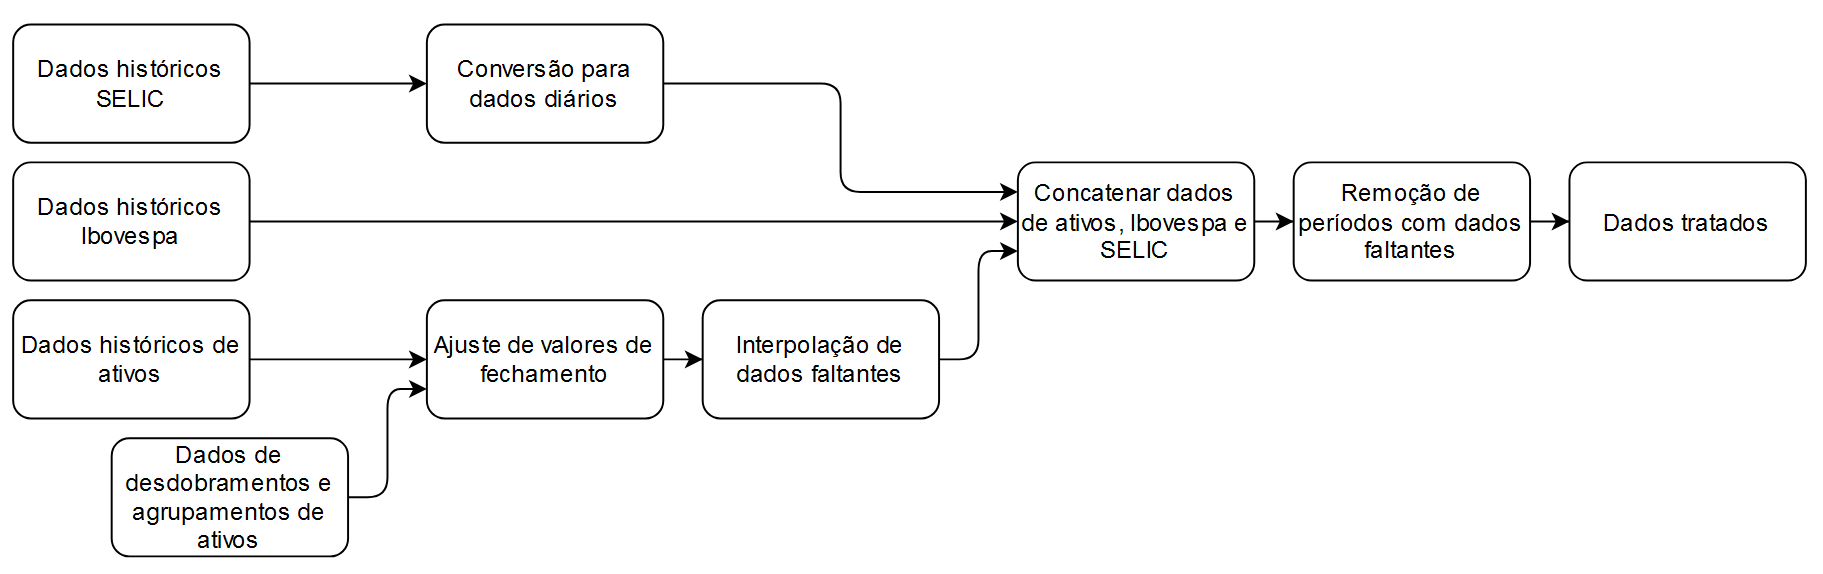
\includegraphics[width=\textwidth]{images/fluxo_tratamento.png}
            \par \footnotesize Fonte: próprio autor.
        \end{figure}
        
    \end{frame}
    \note{Fluxo pré-processamento}
%-------------------------------------------------------




%-------------------------------------------------------
    \begin{frame}{Modelagem}

        \Large

        Desenvolvido módulo onde são preparadas as seguintes combinações.

        \begin{itemize}
            \item Intervalos de tempo: diários, semanais e mensais
            \item Métodos de cálculo de retorno: média simples, médias móveis, médias móveis exponenciais e ARIMA(0,1,1)
            \item Métodos de cálculo de risco: desvio padrão e GARCH(1,1)
        \end{itemize}

        Como exemplo, filtra-se dados de início de semana a partir de 2018 por 60 semanas. Os dados são agrupados por semana, ou seja, o primeiro dia da semana será a referência para o filtro dos dados. Em seguida, são selecionados os valores das datas obtidas, e calcula-se o retorno médio e o desvio padrão dos retornos.
        
    \end{frame}
    \note{Parâmetros, arquitetura}
%-------------------------------------------------------




%-------------------------------------------------------
    \begin{frame}{Otimização de Portfólio}

        \Large

        Modelo proposto a aplicação das seguintes restrições: capital de investimento, custos de operação, cotação e lotes de negociação, rebalanceamento, aversão ao risco e somente posições de compra. 
        
        Este modelo permite responder as seguintes perguntas: quanto dinheiro tem, e quanto aceita perder no intervalo de investimento para obter o máximo retorno?
        
        $\kappa_{j}$ é a variável de decisão, $\delta_{j}$ e $z_{j}$ são as variáveis auxiliares. A descrição segue:
        
        \begin{equation*}
            \begin{aligned}
                \kappa_{j}  \geq 0 \ \in \mathbb{Z} \quad j=1, \ldots, n , \quad & \text{quantidade de lotes} \\
                \delta_{j}  \geq 0 \ \in \mathbb{Z} \quad j=1, \ldots, n , \quad & \text{quantidade de rebalanceamento no lote} \\
                z_{j} \in\{0,1\} \quad j=1, \ldots, n, \quad & \text{1 se o ativo alterar quantidade}
            \end{aligned}
        \end{equation*}

    \end{frame}
    \note{Modelo e restrições}
%-------------------------------------------------------





%-------------------------------------------------------
    \begin{frame}{Otimização de Portfólio}

        Função objetivo, variáveis dependentes, cotação e lotes de negociação:

        \begin{columns}
            \begin{column}{0.5\textwidth}

                \begin{subequations}
                    \label{eq:otimizacao_1}
                    \begin{align}
                        % 
                        & \underset{\kappa}{\text{maximizar}}
                        & & \frac{r_{p}(\kappa) - \frac{r_{f}}{(1+c_{r_{f}}) C_{p}(\kappa)}}{\sigma_{p}(\kappa)} \\
                        % 
                        & \text{sujeito a} \notag \\
                        % 
                        & & & r_{p}(\kappa) = \sum_{j=1}^{n} \kappa_{j} q_{j} \mu_{j} -  \sum_{j=1}^{n} K_{j} \\
                        % 
                        & & & \sigma_{p}(\kappa) = \sqrt{\sum_{j=1}^{n} \sum_{i=1}^{n} \kappa_{j} \kappa_{i} q_{j} q_{i} \sigma_{j} \sigma_{i} \rho_{ij}} \\
                        % 
                        & & & C_{p}(\kappa) = \sum_{j=1}^{n} q_{j}\kappa_{j} + K_{j}
                        % 
                    \end{align}
                \end{subequations}
            \end{column}

            \begin{column}{0.5\textwidth}

                \begin{equation*}
                    \begin{aligned}
                        r_{p} : \quad & \text{retorno da carteira} \\
                        \sigma_{p} : \quad & \text{risco da carteira} \\
                        r_{f} : \quad & \text{retorno livre de risco} \\
                        C_{p} : \quad & \text{capital da carteira} \\
                        c_{r_{f}} : \quad & \text{taxa de imposto para ativo livre de risco} \\
                        q_{j} : \quad & \text{cotação do lote padrão} \\
                        K_{j} : \quad & \text{custo de transação do ativo}
                    \end{aligned}
                \end{equation*}

            \end{column}
        \end{columns}




    \end{frame}
    \note{Restrições reais}
%-------------------------------------------------------






%-------------------------------------------------------
    \begin{frame}{Otimização de Portfólio}

        Restrições de capital, custos de operação e rebalanceamento:

        \begin{columns}
            \begin{column}{0.5\textwidth}

                \begin{subequations}
                    \label{eq:otimizacao_2}
                    \begin{align}
                        & K_{j} = \sum_{j=1}^{n}c_{j}q_{j}\delta_{j} + \sum_{j=1}^{n} f_{j} z_{j}   \\
                        %
                        & C_{0} = \sum_{i=1}^{n}q_{i}\kappa_{i}^{0}+ B \\
                        %
                        & C_{0} \geq C_{p} \\
                        % 
                        &  q_{j}\kappa_{j} \leq z_{j} C_{0} \quad j=1, \ldots, n \text{,} \\
                        % 
                        & \delta_{j} \geq \left( \kappa_{j} -\kappa_{j}^{0} \right) \quad j=1, \ldots, n \\
                        % 
                        & \delta_{j} \geq -\left( \kappa_{j} -\kappa_{j}^{0} \right) \quad j=1, \ldots, n \\
                        % 
                        & \delta_{j} \leq \gamma_{j}z_{j} \quad j=1, \ldots, n
                    \end{align}
                \end{subequations}
            \end{column}

            \begin{column}{0.5\textwidth}

                \begin{equation*}
                    \begin{aligned}
                        f_{j} : \quad & \text{taxa de transação do ativo} \\
                        c_{j} : \quad & \text{custo de transação do ativo} \\
                        \kappa_{j}^{0} : \quad & \text{quantidade inicial de lotes do ativo} \\
                        \gamma_{j} : \quad & \text{quantidade máxima de lotes do ativo}
                    \end{aligned}
                \end{equation*}

            \end{column}
        \end{columns}

    \end{frame}
    \note{Otimizadores}
%-------------------------------------------------------







%-------------------------------------------------------
    \begin{frame}{Otimização de Portfólio}

        Restrições de aversão ao risco:

        \begin{columns}
            \begin{column}{0.5\textwidth}


                \begin{subequations}
                    \label{eq:otimizacao_4}
                    \begin{align}
                        & r_{inv} - \sigma_{inv} Z_{\beta} \geq VaR \\
                        % 
                        & \sigma_{inv} = \sigma_{p} \frac{C_{p}}{C_{0}} \\
                        % 
                        & r_{inv} = \frac{C_{0} - C_{p}}{C_{0}} \frac{r_{f}}{(1+c_{r_{f}})} + \frac{C_{p}}{C_{0}} r_{p}
                    \end{align}
                \end{subequations}

            \end{column}

            \begin{column}{0.5\textwidth}

                \begin{equation*}
                    \begin{aligned}
                        r_{inv} : \quad & \text{retorno do investimento} \\
                        \sigma_{inv} : \quad & \text{risco do investimento} \\
                        VaR : \quad & \text{valor monetário aceitável de perda} \\
                        Z_{\beta} : \quad & \text{quantil da distribuição normal padrão} \\
                        & \quad \text{ ao nível de confiança }\beta.
                    \end{aligned}
                \end{equation*}

            \end{column}
        \end{columns}

    \end{frame}
    \note{Otimizadores}
%-------------------------------------------------------


%-------------------------------------------------------
    \begin{frame}{Otimização de Portfólio}

        \LARGE
        Métodos para otimização:

        \begin{itemize}
            \item Otimização de portfólio sem restrições reais: SLSQP (\citeauthor{kraft1988sqlsp})
            \item Otimização de portfólio com restrições: APOPT (\citeauthor{hedengren2014nonlinear}).
            \item Inicialização do otimizador: Distribuição Dirichlet \cite{yang2022selective}.
            \item Matheurística:  Busca no núcleo (\citeauthor{angelelli2012kernel}).
        \end{itemize}

        
    \end{frame}
    \note{Heurística}
%-------------------------------------------------------





%-------------------------------------------------------
    \begin{frame}{Treinamento de redes neurais}


        
        \begin{columns}
            \begin{column}{0.5\textwidth}

                \begin{figure}[htp]
                    \centering
                    \caption{Fluxograma de redes neurais de RNN com auto atenção.}
                    \label{fig:RNN_SelfAtt}
                    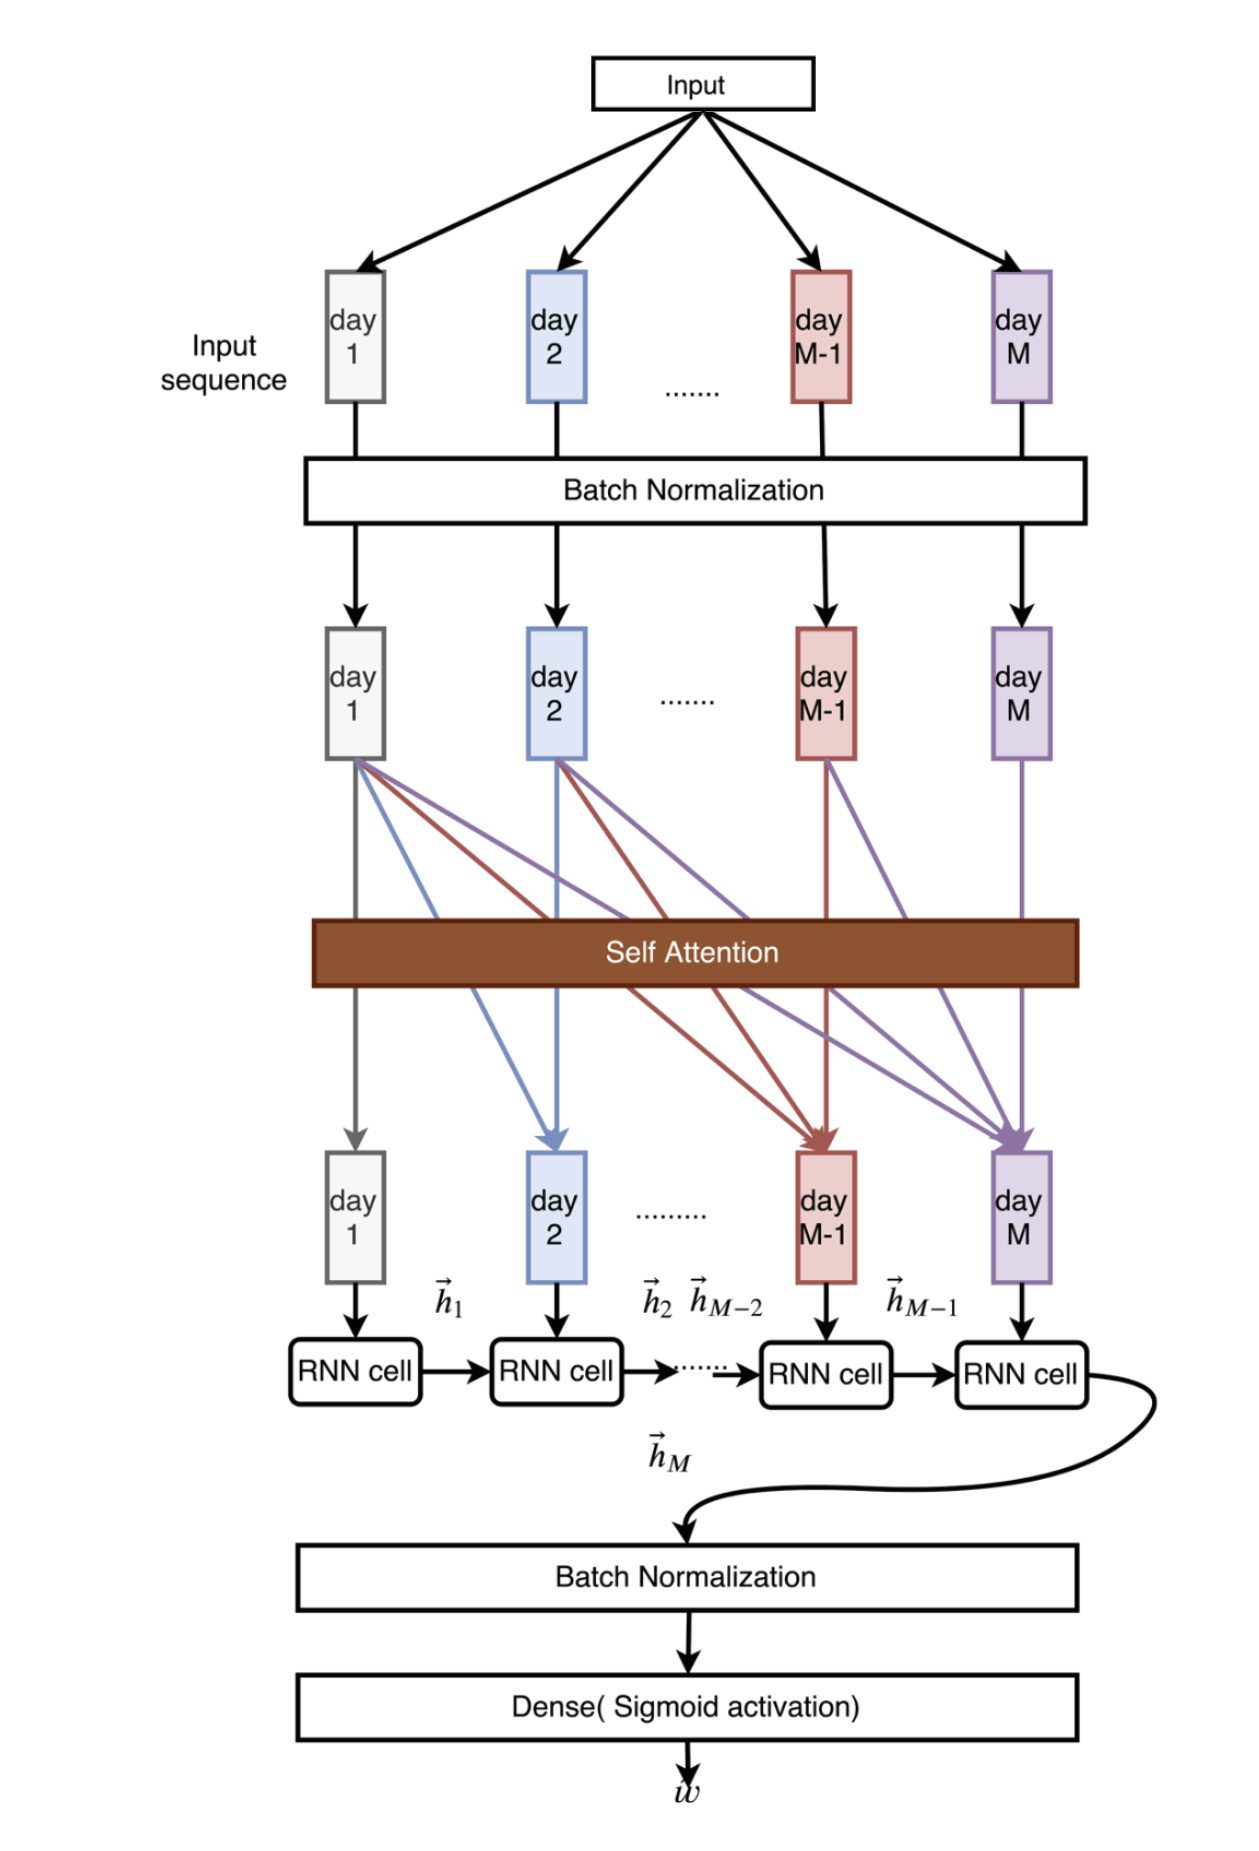
\includegraphics[width=0.55\textwidth]{./images/RNN_SelfAtt.png}
                    \par \footnotesize Fonte: adaptado de \citeauthor{cao2020delafo}.
                \end{figure}


            \end{column}

            \begin{column}{0.5\textwidth}

                \begin{figure}[htp]
                    \centering
                    \caption{Estrutura de rede neural LSTM com auto atenção.}
                    \label{fig:model_lstm_SelfAtt}
                    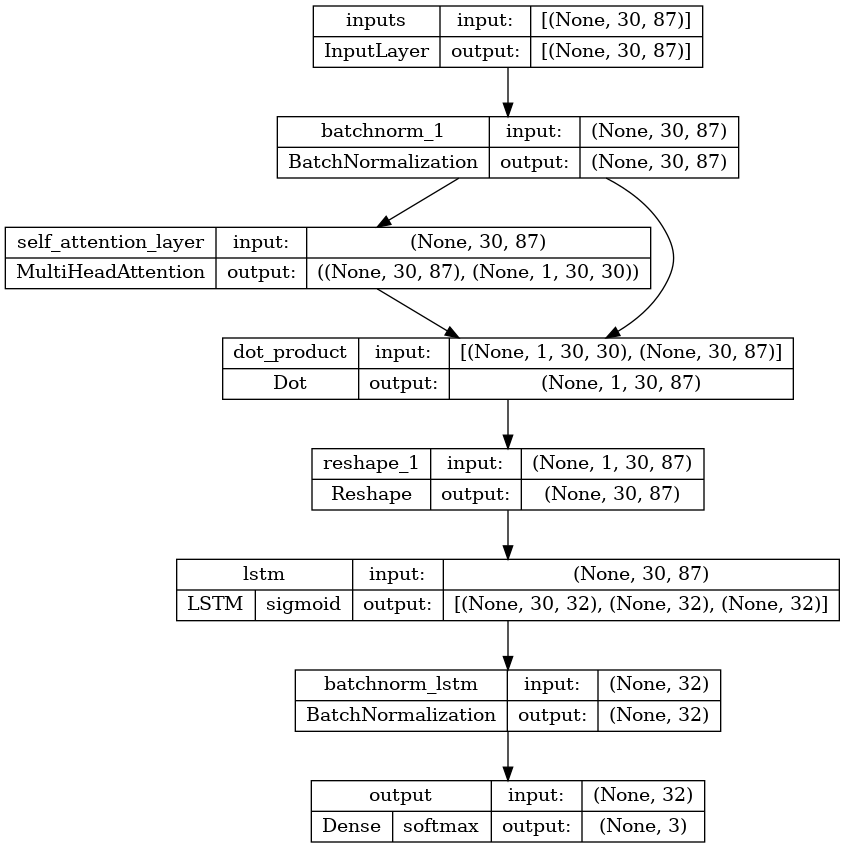
\includegraphics[width=0.65\textwidth]{./images/lstm_selfatt.png}
                    \par \footnotesize Fonte: próprio autor.
                \end{figure}

            \end{column}
        \end{columns}

        
    \end{frame}
    \note{Estruturas de redes RNN e Auto Atenção}
%-------------------------------------------------------




%-------------------------------------------------------
    \begin{frame}{Treinamento de redes neurais}

        
        \begin{columns}
            \begin{column}{0.5\textwidth}

                \begin{figure}[htp]
                    \centering
                    \caption{Fluxograma de redes neurais de RNN com atenção de Bahdanau.}
                    \label{fig:RNN_BauhAtt}
                    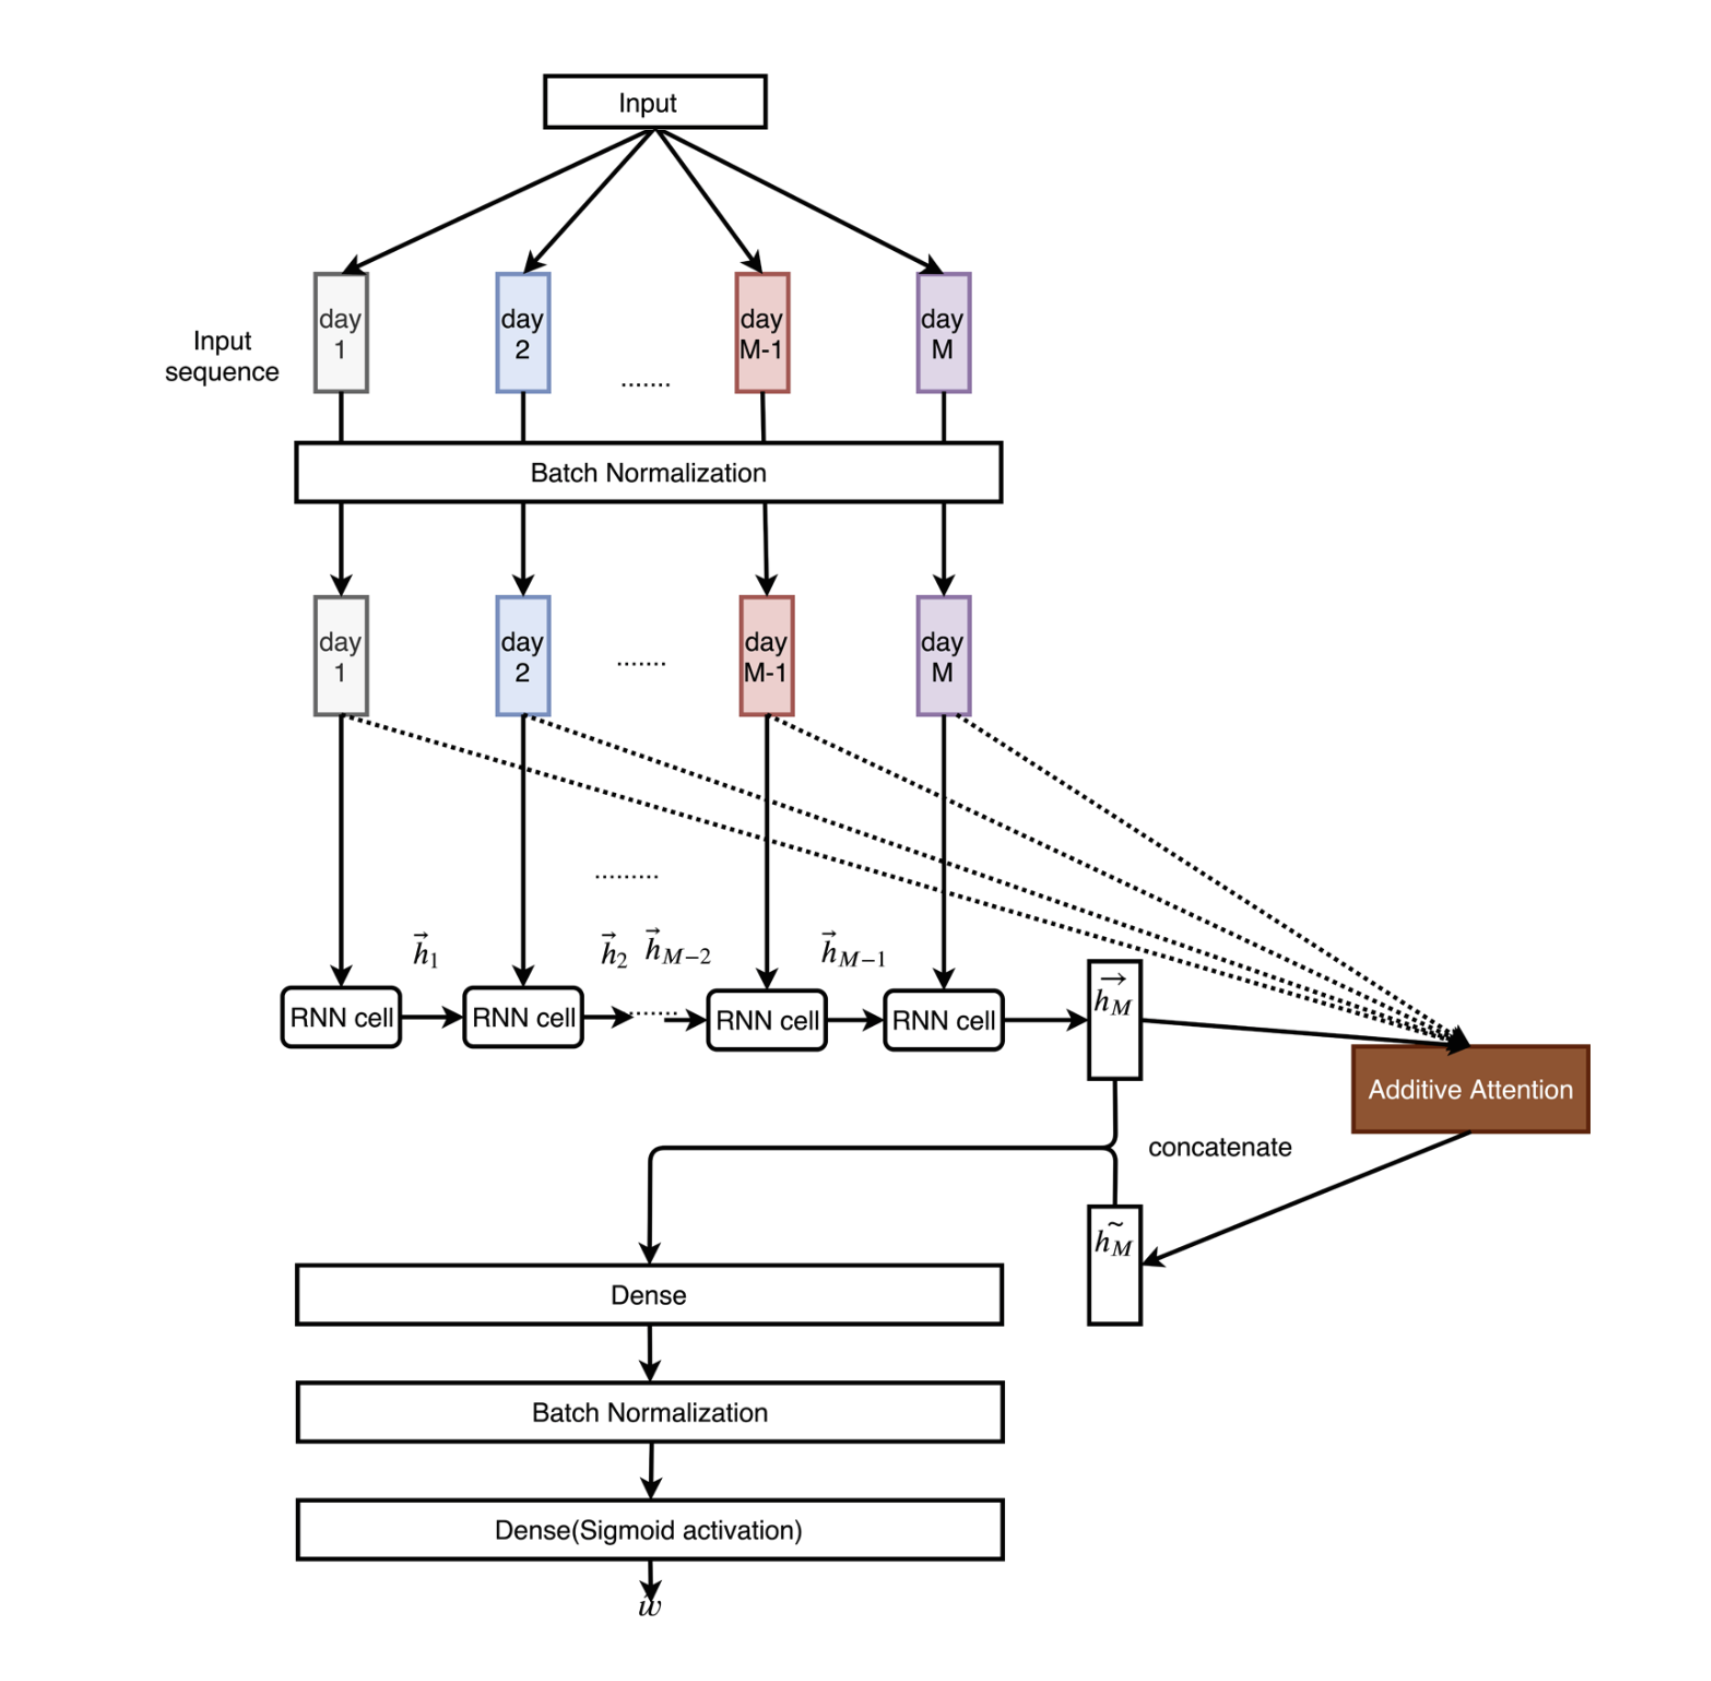
\includegraphics[width=0.8\textwidth]{./images/RNN_AddAtt.png}
                    \par \footnotesize Fonte: adaptado de \citeauthor{cao2020delafo}.
                \end{figure}

            \end{column}

            \begin{column}{0.5\textwidth}

                \begin{figure}[htpb]
                    \centering
                    \caption{Estrutura de rede neural LSTM com atenção de Bahdanau.}
                    \label{fig:model_lstm_BauhAtt}
                    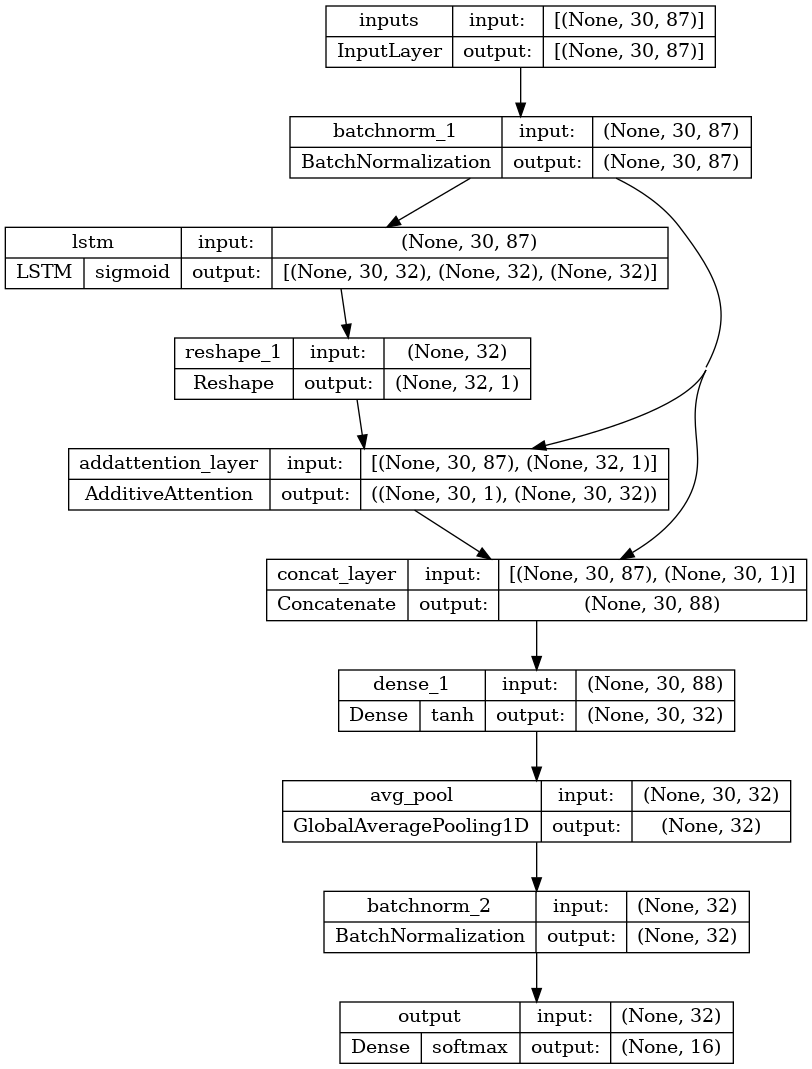
\includegraphics[width=0.6\textwidth]{./images/model_lstm_BauhAtt.png}
                    \par \footnotesize Fonte: próprio autor.
                \end{figure}

            \end{column}
        \end{columns}

        
    \end{frame}
    \note{Estruturas de redes RNN e Atenção de Bahdanau}
%-------------------------------------------------------





%-------------------------------------------------------
    \begin{frame}{Treinamento de redes neurais}


        \begin{columns}
            \begin{column}{0.5\textwidth}

                Período de análise: 09/2018 - 01/2023

                Hiperparâmetros: Hyperband Tuning,

                \begin{itemize}
                    \item Taxa de aprendizagem: $0.0001$ a $1$ distribuídos em função logarítmica reversa.
                    \item Regularização $L_{2}$: $0.0001$ a $1$ distribuídos em função logarítmica reversa.
                    \item Épocas: 30.
                \end{itemize}

                Validação cruzada: 10 \textit{folds} com lacunas de duas partes anteriores e uma parte posterior.

                
                Função de perda: entropia cruzada categórica.
                
                Métrica: acurácia.

            \end{column}

            \begin{column}{0.5\textwidth}


                \begin{figure}[htp]
                    \centering
                    \caption{Validação cruzada com lacunas.}
                    \label{fig:cross_validation}
                    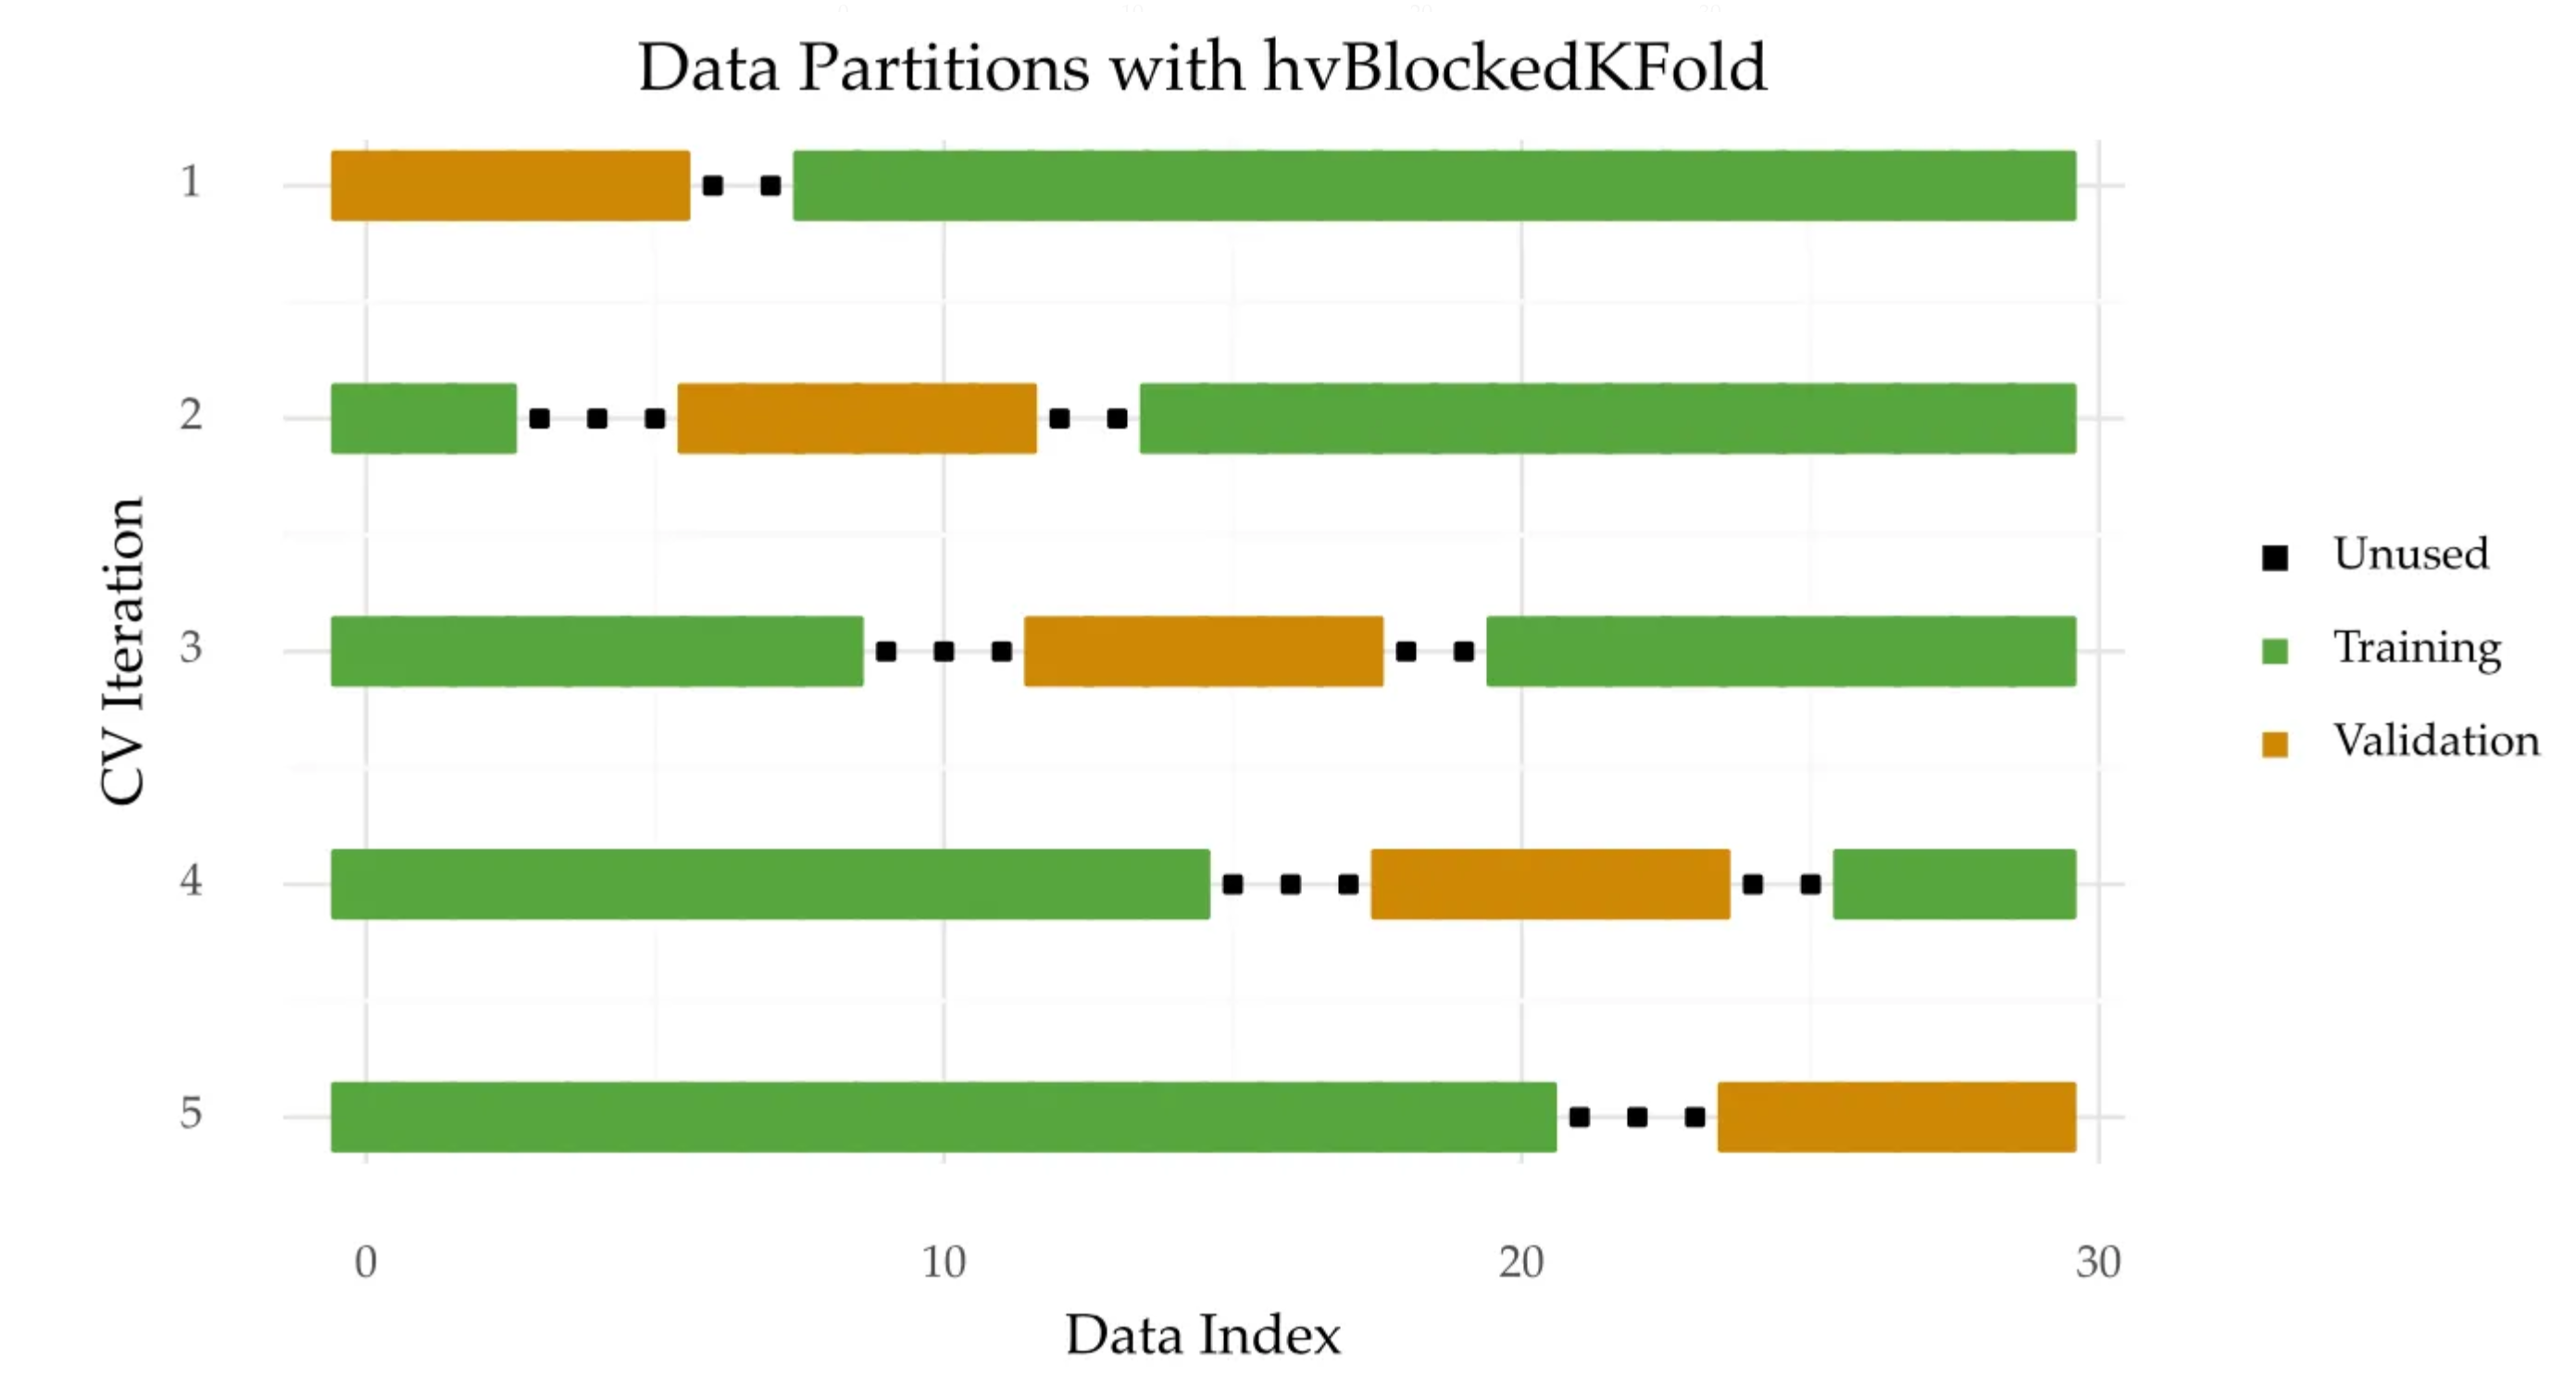
\includegraphics[width=0.8\textwidth]{./images/cross_validation.png}
                    \par \footnotesize Fonte: \citeauthor{Cerqueira2023}.
                \end{figure}

            \end{column}
        \end{columns}

    \end{frame}
    \note{Hiperparâmetros, e separação dos dados}
%-------------------------------------------------------




%-------------------------------------------------------
    \begin{frame}{Validação de redes neurais}

        Período de análise: 09/2018 - 07/2023

        Dados de entrada: bloco dos últimos 30 dias de preços de fechamento ajustado de 87 ativos do Ibovespa.

        Divisão dos dados:

        \begin{itemize}
            \item 90\% para treinamento (validação cruzada), 1078 amostras.
            \item 10\% para teste, 120 amostras.
        \end{itemize}

        Atributos alvo: melhor carteira no próximo período dentre 3 carteiras otimizadas pelo índice Sharpe.

        \begin{itemize}
            \item Parâmetros de modelagem: média simples e desvio padrão.
            \item Intervalo de tempo para retorno: últimos 15, 30 e 60 dias.
            \item Intervalo de ajuste da otimização: diário.
        \end{itemize}
        
    \end{frame}
    \note{Cross validation e métricas}
%-------------------------------------------------------
